\icode[magenta]{N23Q-EME-SI-L4-261121-001}
\nceeID[unkown]{2023海南}{unkown}
如图所示，一光滑绝缘轨道水平放置，直径上有\(A\)、\(B\)两点，\(AO=\) \,\qty{2}{cm}，\(OB =\) \,\qty{4}{cm}，在\(AB\)固定两个带电量分别为\(Q_1\)、\(Q_2\)的正电荷，现有一个带正电小球静置于轨道内侧\(P\)点(小球可视为点电荷)，已知\(AP:BP=n:1\)，试求\(Q_1:Q_2\)是多少\paren[]

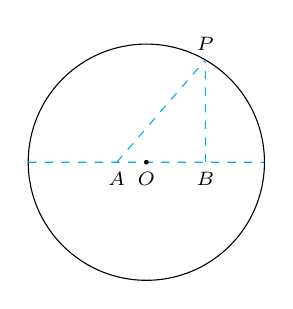
\begin{tikzpicture}[>=stealth,font=\scriptsize]
	\draw (0,0)node[below]{\(O\)} circle(1.5);
	\draw[dashed,cyan] (-1.5,0)--(1.5,0) (.75,0)node[below,black]{\(B\)}--(.75,{.75*sqrt(3)}) (-.375,0)node[below,black]{\(A\)}--(.75,{.75*sqrt(3)})node[above,black]{\(P\)};
	\fill (0,0) circle(.03);
\end{tikzpicture}
\begin{choices}
	\item \(2n^2:1\)
	\item \(4n^2:1\)
	\item \(2n^3:1\)
	\item \(4n^3:1\)
\end{choices}
\begin{answer}
	
\end{answer}